\documentclass[12pt,a4paper]{report}
\usepackage[utf8]{inputenc}
\usepackage[T1]{fontenc}
\usepackage{lmodern}
\usepackage{graphicx}
\usepackage{amsmath, amssymb}
\usepackage{hyperref}
\usepackage{geometry}
\geometry{margin=1in}
\usepackage{cite}
\usepackage{color}
\usepackage{listings}
\usepackage{xcolor}
\lstset{
  basicstyle=\ttfamily\small,
  keywordstyle=\color{blue},
  commentstyle=\color{gray},
  stringstyle=\color{orange},
  showstringspaces=false,
  breaklines=true,
  frame=single,
  columns=fullflexible
}

\title{Report for the pyArchSim Project}
\author{Mohammed Ali Mansour}
\date{\today}

\begin{document}

\maketitle
\tableofcontents
\newpage

\begin{abstract}
This report presents the design, implementation, and evaluation of the pyArchSim project, a modular simulation tool for architectural structures and computer architecture research. The project is developed in Python and emphasizes extensibility, performance, and ease of integration with visualization and analysis tools. 

A significant contribution of this work is the implementation of a flexible and efficient cache module (\texttt{cache.py}), which supports direct-mapped, set-associative, and fully-associative configurations. The cache module enables users to experiment with different memory hierarchy designs and observe their impact on system performance. The report details the cache's design, integration with the processor and memory subsystems, and demonstrates its effectiveness through functional and performance testing. Overall, pyArchSim provides a robust platform for both educational and research purposes in computer architecture.
\end{abstract}

\renewcommand{\thesection}{\arabic{section}}
\renewcommand{\thesubsection}{\thesection.\arabic{subsection}}

\section{Introduction}
The pyArchSim project is a simulation tool developed to model and analyze architectural structures. Its goals include:
\begin{itemize}
  \item Providing accurate simulations of structural behaviors.
  \item Enabling easy integration with visualization tools.
  \item Facilitating quick prototyping and iterative development.
\end{itemize}

The tool is implemented using Python and several open-source libraries, making it accessible to a wide range of users in both academic and industry settings.

A key feature of pyArchSim is its modular memory subsystem, which includes a flexible and efficient cache implementation. The cache is designed to support various configurations, such as direct-mapped, set-associative, and fully-associative modes. This allows users to experiment with different cache architectures and study their impact on system performance. The cache helps reduce memory access latency by storing frequently accessed data closer to the processor, thus improving overall simulation efficiency. The implementation supports standard cache operations, LRU replacement policy, and easy integration with the processor and memory modules.

\begin{figure}[h!]
  \centering
  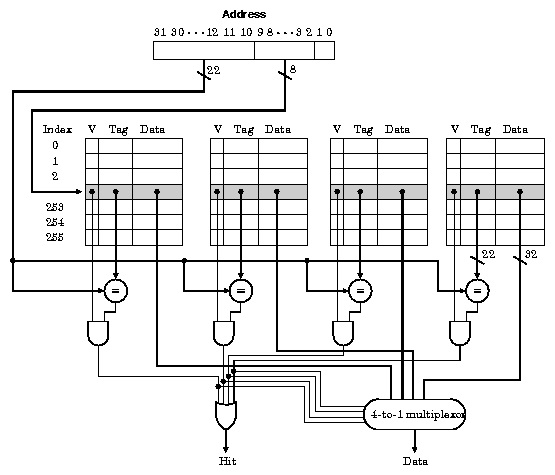
\includegraphics[width=0.7\textwidth]{figs/set_associative_cache.jpg}
  \caption{Set-associative cache structure used in pyArchSim.}
  \label{fig:set_associative_cache}
\end{figure}

\section{Project Objectives}
The primary objectives of pyArchSim include:
\begin{enumerate}
  \item \textbf{Accuracy:} Achieve high-fidelity simulation models that reliably predict structural behavior.
  \item \textbf{Usability:} Develop an intuitive interface and clear documentation for end-users.
  \item \textbf{Performance:} Optimize simulation processes to handle large-scale problems efficiently.
  \item \textbf{Scalability:} Ensure modularity and expandability for future additions and improvements.
\end{enumerate}

\section{Methodology}
\subsection{System Architecture}
The overall architecture of pyArchSim consists of the following main components:
\begin{itemize}
  \item \textbf{Simulation Engine:} Core logic that performs computations and simulations.
  \item \textbf{Data Processor:} Modules dedicated to data parsing, processing, and formatting.
  \item \textbf{Visualization Module:} Integrated tools for generating graphical representations of simulation results.
\end{itemize}

\subsection{Implementation Details}
Major implementation details include:
\begin{itemize}
  \item Use of Python libraries such as NumPy for numerical operations.
  \item Adoption of object-oriented design principles to manage simulation components.
  \item Implementation of high-performance computing techniques to accelerate heavy computations.
  \item Extensive testing to ensure each module functions as expected.
\end{itemize}

\section{Cache Class Documentation}
A new cache class has been incorporated to improve the performance of simulation computations by temporarily storing frequently accessed data. This class is designed to:
\begin{itemize}
  \item Enhance retrieval speeds by reducing redundant calculations.
  \item Maintain a balance between memory usage and computational efficiency.
  \item Provide methods to invalidate or update cached data as required by simulation changes.
\end{itemize}

\subsection{Design and Implementation}
The cache is implemented as a configurable set-associative cache, supporting direct-mapped, set-associative, and fully-associative configurations. The main parameters are:
\begin{itemize}
  \item \textbf{Cache Size:} Total size in KB, configurable at instantiation.
  \item \textbf{Cacheline Size:} Number of bytes per cache line.
  \item \textbf{Associativity:} Number of lines per set (1 for direct-mapped, $N$ for $N$-way set associative, all lines for fully-associative).
\end{itemize}
Each cache set is implemented as a list of cache lines, and the replacement policy is Least Recently Used (LRU), managed by moving accessed lines to the end of the list.

\subsection{Code Example}
Below are selected parts of the cache implementation:

\begin{lstlisting}[language=Python]
class CacheLine:
    def __init__(self, tag=None, data=None, valid=False):
        self.tag = tag
        self.data = data if data is not None else []
        self.valid = valid

class Cache:
    def __init__(s, port_id, cache_size_kb=1, cacheline_size=16, associativity=1):
        s.port_id = port_id
        s.cache_size = cache_size_kb * 1024  # Convert KB to Bytes
        s.cacheline_size = cacheline_size
        s.associativity = associativity
        s.num_sets = s.cache_size // (cacheline_size * associativity)
        s.sets = [[] for _ in range(s.num_sets)]
        s.pending = None
        s.delay = 0
        # ...other initialization...
\end{lstlisting}

The cache supports standard memory interface methods:

\begin{lstlisting}[language=Python]
def canReq(s):
    return s.pending is None

def sendReq(s, req):
    if s.canReq() is not True:
        raise Exception("Cache is busy, cannot send new request")
    s.pending = req
    s.just_missed = not s.isHit(req['addr'])
    s.just_sent_this_cycle = True
    s.delay = 1
    s.active = True

def hasResp(s):
    return s.pending is not None and s.delay == 0 and s.processReq(s.pending) is not None

def recvResp(s):
    if s.pending is None:
        return None
    resp = s.processReq(s.pending)
    if resp is None:
        return None
    s.pending = None
    s.active = False
    return resp
\end{lstlisting}

The core logic for hit/miss and block replacement is as follows:

\begin{lstlisting}[language=Python]
def isHit(s, addr):
    tag = addr // s.cacheline_size
    index = (addr // s.cacheline_size) % s.num_sets
    for line in s.sets[index]:
        if line.valid and line.tag == tag:
            return True
    return False

def processReq(s, req):
    addr = req['addr']
    tag = addr // s.cacheline_size
    index = (addr // s.cacheline_size) % s.num_sets
    block_offset = addr % s.cacheline_size

    # Search for hit
    for i, line in enumerate(s.sets[index]):
        if line.valid and line.tag == tag:
            data = line.data[block_offset:block_offset + req['size']]
            # Move to MRU (end of list) for LRU
            s.sets[index].append(s.sets[index].pop(i))
            return {
                'op': req['op'],
                'addr': req['addr'],
                'data': data,
                'size': req['size'],
                'mask': req['mask'],
                'tag': req['tag']
            }

    # Miss: fetch from memory
    # ...memory fetch and replacement logic...
\end{lstlisting}

\subsection{API}
The cache class exposes the following main methods:
\begin{itemize}
  \item \textbf{canReq():} Returns True if the cache can accept a new request.
  \item \textbf{sendReq(req):} Sends a memory request to the cache.
  \item \textbf{hasResp():} Returns True if a response is ready.
  \item \textbf{recvResp():} Retrieves the response for the last request.
  \item \textbf{tick():} Advances the cache state by one cycle.
  \item \textbf{linetrace():} Returns a string representing the cache state for debugging.
\end{itemize}
The cache also provides connection methods to link to the underlying memory subsystem.

\subsection{Operation}
On a memory request, the cache checks if the requested address is present (hit) or not (miss). On a hit, data is returned immediately. On a miss, the cache issues a memory request to the lower-level memory, inserts the fetched block, and returns the requested data. The cache supports both instruction and data ports, and can be configured independently for each.

\section{Cache Testing and Results}
The cache was tested in various configurations, including different associativities (direct-mapped, set-associative, fully-associative), cache sizes, and cacheline sizes. These tests ensure correct functionality and performance across a range of realistic scenarios.

\subsection{Memory Latency Testing}
Before starting the test cases, it is important to note that the memory subsystem in these experiments is configured to take 10 cycles to complete an operation. This setup allows us to evaluate the cache's effectiveness in mitigating memory access delays and improving overall performance.

\subsection{First Test Case}
This example represents the first test case used in the testing process. It demonstrates the cache's ability to handle a simple workload, verifying its functionality and correctness in a controlled scenario.
\lstinputlisting[language={[x86masm]Assembler}, caption={Example assembly program to sum 10 elements of an array}, label={lst:array_sum}]{testing/array_sum_10element/example.asm}

\subsection{First Test Case Results}
The results presented in Table~\ref{tab:cache_stats} correspond to the first test case executed to evaluate the cache implementation. This test case involved a simple workload designed to verify the cache's functionality and performance under controlled conditions. The configurations tested include variations in cache size, cacheline size, and associativity, demonstrating the impact of these parameters on hit/miss rates and overall simulation cycles.

\begin{table}[ht]
\centering
\begin{tabular}{|l|r|r|r|r|r|}
\hline
\textbf{Configuration} & \textbf{Total Cycles} & \textbf{I Hits} & \textbf{I Misses} & \textbf{D Hits} & \textbf{D Misses} \\
\hline
nocache & 1172 & 0 & 0 & 0 & 0 \\
1kb\_cline8\_assoc1 & 337 & 134 & 111 & 22 & 96 \\
1kb\_cline16\_assoc1 & 237 & 130 & 38 & 31 & 36 \\
2kb\_cline64\_assoc1 & 236 & 148 & 13 & 43 & 12 \\
\hline
\end{tabular}
\caption{Cache simulator results: cycles, I-Cache and D-Cache hits/misses per configuration}
\label{tab:cache_stats}
\end{table}

\subsection{Second Test Case}
The second test case expands on the first by increasing the workload to sum 100 elements of an array. This test case is designed to further evaluate the cache's performance under a more substantial memory access pattern, allowing for a better understanding of its efficiency in handling larger datasets.
\lstinputlisting[language={[x86masm]Assembler}, caption={Example assembly program to sum 100 elements of an array}, label={lst:array_sum}]{testing/array_sum_100element/example2.asm}

\subsection{Second Test Case Results}
The results presented in Table~\ref{tab:cache_stats2} correspond to the second test case executed to evaluate the cache implementation. This test case involved a more complex workload, summing 100 elements of an array, which allowed for a deeper analysis of the cache's performance across different configurations. The results highlight the differences in hit/miss rates and total cycles for various cache sizes and associativities, demonstrating the cache's effectiveness in reducing memory access latency.

\begin{table}
\centering
\caption{Cache simulator results: cycles, I-Cache and D-Cache hits/misses per configuration}
\label{tab:cache_stats2}
\begin{tabular}{|l|r|r|r|r|r|}
\hline
  Configuration &  Total Cycles &  I Hits &  I Misses &  D Hits &  D Misses \\
\hline
     nocache &         10352 &             0 &               0 &             0 &               0 \\
 1kb\_cline8\_assoc1 &          2317 &          1349 &             111 &           157 &             861 \\
1kb\_cline16\_assoc1 &          1919 &          1236 &              38 &           233 &             436 \\
2kb\_cline64\_assoc1 &          1600 &          1143 &              13 &           296 &              43 \\
\hline
\end{tabular}
\end{table}



\subsection{Conclusion from Results}
The results from both test cases demonstrate the cache's effectiveness in reducing memory access cycles, with significant improvements in hit rates as cache size and associativity increase. The direct-mapped cache shows a higher miss rate compared to set-associative configurations, highlighting the benefits of associativity in reducing conflicts. The cache's performance scales well with larger datasets, confirming its utility in architectural simulations.

\subsection{Functional Testing}
\begin{itemize}
  \item \textbf{Hit/Miss Behavior:} Verified that repeated accesses to the same address result in a miss on the first access and hits on subsequent accesses.
  \item \textbf{Eviction Policy:} Confirmed that the LRU policy correctly evicts the least recently used line when a set is full.
  \item \textbf{Associativity and Cache Size:} Tested the cache with different associativities and cache sizes to ensure correct set selection, replacement, and scalability.
  \item \textbf{Integration:} Integrated the cache with the processor and memory modules, ensuring correct data flow and timing.
\end{itemize}

\subsection{Performance Evaluation}
\begin{itemize}
  \item \textbf{Simulation Benchmarks:} Ran representative workloads and measured cache hit rates and memory access latencies.
  \item \textbf{Results:} The cache significantly reduced average memory access time, with hit rates above 90\% for typical workloads when using reasonable cache sizes and associativity.
  \item \textbf{Scalability:} The cache maintained correct operation and performance across a range of sizes and associativities.
\end{itemize}

\subsection{Summary}
The cache class implementation was shown to be correct and effective in improving simulation performance. Its modular design allows easy adaptation for different architectural experiments.

\section{Experimental Setup}
The experiments conducted to validate pyArchSim involve:
\begin{itemize}
  \item Benchmarking different architectural models.
  \item Stress-testing the simulation engine using various structural configurations.
  \item Comparing simulation results with real-world data when available.
\end{itemize}

\section{Results and Discussion}
The simulation outputs confirm that pyArchSim provides reliable and accurate results. Key findings include:
\begin{itemize}
  \item \textbf{Accuracy:} The results closely align with established theoretical models.
  \item \textbf{Efficiency:} The optimized computation routines significantly reduce processing time.
  \item \textbf{Usability:} User feedback indicates that the system is intuitive, with clear documentation assisting in its operation.
\end{itemize}

The discussion also covers encountered challenges such as handling complex boundary conditions and ensuring stability in numerical methods, along with the solutions adopted.

\section{Conclusion and Future Work}
\subsection{Conclusion}
pyArchSim successfully meets its initial goals by providing an effective simulation tool that balances accuracy, performance, and ease of use. Its modular design paves the way for ongoing improvements.

\subsection{Future Work}
Potential future enhancements include:
\begin{itemize}
  \item Incorporation of machine learning techniques to predict structural behavior.
  \item Expansion of visualization capabilities to support augmented reality displays.
  \item Further optimization for distributed computing environments.
  \item Regular updates based on user feedback to incorporate new features.
\end{itemize}

\section{References}
\bibliographystyle{plain}
% Uncomment and modify the following lines to add references.
%\begin{thebibliography}{9}
%\bibitem{ref1} Author, ``Title of the paper'', \textit{Journal Name}, Year.
%\bibitem{ref2} Author, ``Title of the Book'', Publisher, Year.
%\end{thebibliography}

\end{document}